\section*{Questão 9}

\paragraph{}Nas seções precedentes o cálculo das parametrizações de cada coordenada
foram independentes umas das outras. Dessa forma acrescentar a terceira coordenada
é trivial, basta repetir o mesmo processo. O resultado é apresentado nos gráficos a 
seguir. A curva é vista de dois ângulos para que se possa melhor perceber o ajuste 
tridimensional.

\FloatBarrier
\begin{figure}[!htp]
	\begin{subfigure}[!htp]{0.5\textwidth}
	% GNUPLOT: LaTeX picture with Postscript
\begingroup
  \fontfamily{phv}%
  \selectfont
\definecolor{t}{rgb}{0.5,0.5,0.5}
  \makeatletter
  \providecommand\color[2][]{%
    \GenericError{(gnuplot) \space\space\space\@spaces}{%
      Package color not loaded in conjunction with
      terminal option `colourtext'%
    }{See the gnuplot documentation for explanation.%
    }{Either use 'blacktext' in gnuplot or load the package
      color.sty in LaTeX.}%
    \renewcommand\color[2][]{}%
  }%
  \providecommand\includegraphics[2][]{%
    \GenericError{(gnuplot) \space\space\space\@spaces}{%
      Package graphicx or graphics not loaded%
    }{See the gnuplot documentation for explanation.%
    }{The gnuplot epslatex terminal needs graphicx.sty or graphics.sty.}%
    \renewcommand\includegraphics[2][]{}%
  }%
  \providecommand\rotatebox[2]{#2}%
  \@ifundefined{ifGPcolor}{%
    \newif\ifGPcolor
    \GPcolortrue
  }{}%
  \@ifundefined{ifGPblacktext}{%
    \newif\ifGPblacktext
    \GPblacktextfalse
  }{}%
  % define a \g@addto@macro without @ in the name:
  \let\gplgaddtomacro\g@addto@macro
  % define empty templates for all commands taking text:
  \gdef\gplbacktext{}%
  \gdef\gplfronttext{}%
  \makeatother
  \ifGPblacktext
    % no textcolor at all
    \def\colorrgb#1{}%
    \def\colorgray#1{}%
  \else
    % gray or color?
    \ifGPcolor
      \def\colorrgb#1{\color[rgb]{#1}}%
      \def\colorgray#1{\color[gray]{#1}}%
      \expandafter\def\csname LTw\endcsname{\color{white}}%
      \expandafter\def\csname LTb\endcsname{\color{black}}%
      \expandafter\def\csname LTa\endcsname{\color{black}}%
      \expandafter\def\csname LT0\endcsname{\color[rgb]{1,0,0}}%
      \expandafter\def\csname LT1\endcsname{\color[rgb]{0,1,0}}%
      \expandafter\def\csname LT2\endcsname{\color[rgb]{0,0,1}}%
      \expandafter\def\csname LT3\endcsname{\color[rgb]{1,0,1}}%
      \expandafter\def\csname LT4\endcsname{\color[rgb]{0,1,1}}%
      \expandafter\def\csname LT5\endcsname{\color[rgb]{1,1,0}}%
      \expandafter\def\csname LT6\endcsname{\color[rgb]{0,0,0}}%
      \expandafter\def\csname LT7\endcsname{\color[rgb]{1,0.3,0}}%
      \expandafter\def\csname LT8\endcsname{\color[rgb]{0.5,0.5,0.5}}%
    \else
      % gray
      \def\colorrgb#1{\color{black}}%
      \def\colorgray#1{\color[gray]{#1}}%
      \expandafter\def\csname LTw\endcsname{\color{white}}%
      \expandafter\def\csname LTb\endcsname{\color{black}}%
      \expandafter\def\csname LTa\endcsname{\color{black}}%
      \expandafter\def\csname LT0\endcsname{\color{black}}%
      \expandafter\def\csname LT1\endcsname{\color{black}}%
      \expandafter\def\csname LT2\endcsname{\color{black}}%
      \expandafter\def\csname LT3\endcsname{\color{black}}%
      \expandafter\def\csname LT4\endcsname{\color{black}}%
      \expandafter\def\csname LT5\endcsname{\color{black}}%
      \expandafter\def\csname LT6\endcsname{\color{black}}%
      \expandafter\def\csname LT7\endcsname{\color{black}}%
      \expandafter\def\csname LT8\endcsname{\color{black}}%
    \fi
  \fi
  \setlength{\unitlength}{0.0500bp}%
  \begin{picture}(7936.00,5668.00)%
    \gplgaddtomacro\gplbacktext{%
      \csname LTb\endcsname%
      \put(1002,1472){\makebox(0,0){\strut{} 0}}%
      \put(1611,1363){\makebox(0,0){\strut{} 0.2}}%
      \put(2219,1254){\makebox(0,0){\strut{} 0.4}}%
      \put(2828,1145){\makebox(0,0){\strut{} 0.6}}%
      \put(3436,1036){\makebox(0,0){\strut{} 0.8}}%
      \put(4044,926){\makebox(0,0){\strut{} 1}}%
      \put(4652,817){\makebox(0,0){\strut{} 1.2}}%
      \put(4833,867){\makebox(0,0){\strut{}-1}}%
      \put(5024,970){\makebox(0,0){\strut{} 0}}%
      \put(5216,1074){\makebox(0,0){\strut{} 1}}%
      \put(5408,1177){\makebox(0,0){\strut{} 2}}%
      \put(5599,1280){\makebox(0,0){\strut{} 3}}%
      \put(5791,1383){\makebox(0,0){\strut{} 4}}%
      \put(5982,1486){\makebox(0,0){\strut{} 5}}%
      \put(6174,1589){\makebox(0,0){\strut{} 6}}%
      \put(6366,1692){\makebox(0,0){\strut{} 7}}%
      \put(6557,1796){\makebox(0,0){\strut{} 8}}%
      \put(6749,1899){\makebox(0,0){\strut{} 9}}%
      \put(6941,2002){\makebox(0,0){\strut{} 10}}%
      \put(963,2307){\makebox(0,0)[r]{\strut{} 0}}%
      \put(963,2458){\makebox(0,0)[r]{\strut{} 1}}%
      \put(963,2609){\makebox(0,0)[r]{\strut{} 2}}%
      \put(963,2760){\makebox(0,0)[r]{\strut{} 3}}%
      \put(963,2912){\makebox(0,0)[r]{\strut{} 4}}%
      \put(963,3062){\makebox(0,0)[r]{\strut{} 5}}%
      \put(963,3213){\makebox(0,0)[r]{\strut{} 6}}%
      \put(963,3364){\makebox(0,0)[r]{\strut{} 7}}%
      \put(963,3516){\makebox(0,0)[r]{\strut{} 8}}%
      \put(963,3667){\makebox(0,0)[r]{\strut{} 9}}%
      \put(963,3818){\makebox(0,0)[r]{\strut{} 10}}%
      \put(3968,5325){\makebox(0,0){\strut{}Ajuste com Splines 3D}}%
    }%
    \gplgaddtomacro\gplfronttext{%
      \put(5009,630){\makebox(0,0)[r]{\strut{}splines3D}}%
      \csname LTb\endcsname%
      \put(5009,450){\makebox(0,0)[r]{\strut{}data points}}%
      \csname LTb\endcsname%
      \put(2388,939){\makebox(0,0){\strut{}t}}%
      \put(6706,1299){\makebox(0,0){\strut{}y(t)}}%
      \put(7356,2538){\makebox(0,0)[l]{\strut{} 0}}%
      \put(7356,2706){\makebox(0,0)[l]{\strut{} 1}}%
      \put(7356,2875){\makebox(0,0)[l]{\strut{} 2}}%
      \put(7356,3044){\makebox(0,0)[l]{\strut{} 3}}%
      \put(7356,3213){\makebox(0,0)[l]{\strut{} 4}}%
      \put(7356,3382){\makebox(0,0)[l]{\strut{} 5}}%
      \put(7356,3550){\makebox(0,0)[l]{\strut{} 6}}%
      \put(7356,3719){\makebox(0,0)[l]{\strut{} 7}}%
      \put(7356,3888){\makebox(0,0)[l]{\strut{} 8}}%
      \put(7356,4057){\makebox(0,0)[l]{\strut{} 9}}%
      \put(7356,4226){\makebox(0,0)[l]{\strut{} 10}}%
    }%
    \gplbacktext
    \put(0,0){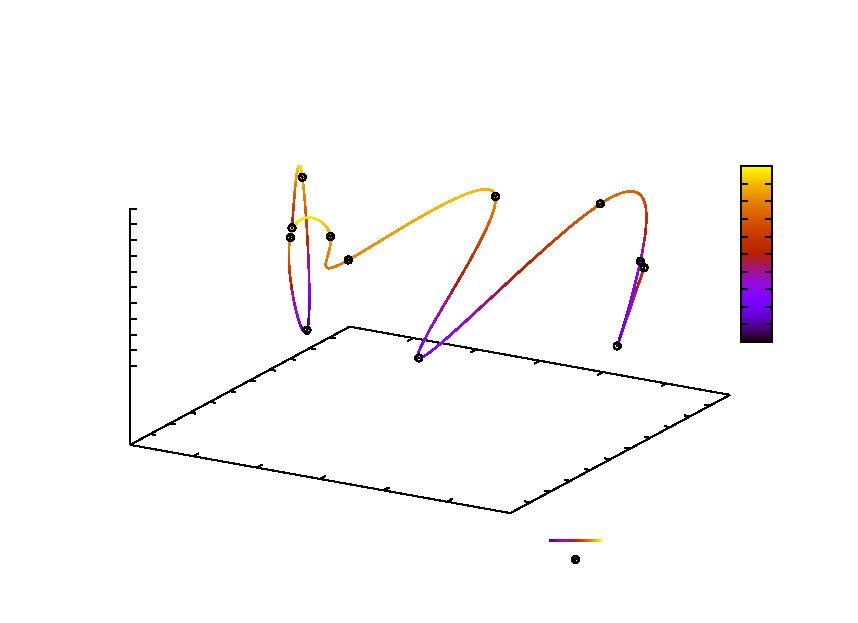
\includegraphics{./../LaTeX/graph/quest9-1}}%
    \gplfronttext
  \end{picture}%
\endgroup

	\caption{Interpolação com splines 3D }
	\label{fig:quest9-1}
	\end{subfigure}
	
	\begin{subfigure}[!htp]{0.5\textwidth}	
	% GNUPLOT: LaTeX picture with Postscript
\begingroup
  \fontfamily{phv}%
  \selectfont
\definecolor{t}{rgb}{0.5,0.5,0.5}
  \makeatletter
  \providecommand\color[2][]{%
    \GenericError{(gnuplot) \space\space\space\@spaces}{%
      Package color not loaded in conjunction with
      terminal option `colourtext'%
    }{See the gnuplot documentation for explanation.%
    }{Either use 'blacktext' in gnuplot or load the package
      color.sty in LaTeX.}%
    \renewcommand\color[2][]{}%
  }%
  \providecommand\includegraphics[2][]{%
    \GenericError{(gnuplot) \space\space\space\@spaces}{%
      Package graphicx or graphics not loaded%
    }{See the gnuplot documentation for explanation.%
    }{The gnuplot epslatex terminal needs graphicx.sty or graphics.sty.}%
    \renewcommand\includegraphics[2][]{}%
  }%
  \providecommand\rotatebox[2]{#2}%
  \@ifundefined{ifGPcolor}{%
    \newif\ifGPcolor
    \GPcolortrue
  }{}%
  \@ifundefined{ifGPblacktext}{%
    \newif\ifGPblacktext
    \GPblacktextfalse
  }{}%
  % define a \g@addto@macro without @ in the name:
  \let\gplgaddtomacro\g@addto@macro
  % define empty templates for all commands taking text:
  \gdef\gplbacktext{}%
  \gdef\gplfronttext{}%
  \makeatother
  \ifGPblacktext
    % no textcolor at all
    \def\colorrgb#1{}%
    \def\colorgray#1{}%
  \else
    % gray or color?
    \ifGPcolor
      \def\colorrgb#1{\color[rgb]{#1}}%
      \def\colorgray#1{\color[gray]{#1}}%
      \expandafter\def\csname LTw\endcsname{\color{white}}%
      \expandafter\def\csname LTb\endcsname{\color{black}}%
      \expandafter\def\csname LTa\endcsname{\color{black}}%
      \expandafter\def\csname LT0\endcsname{\color[rgb]{1,0,0}}%
      \expandafter\def\csname LT1\endcsname{\color[rgb]{0,1,0}}%
      \expandafter\def\csname LT2\endcsname{\color[rgb]{0,0,1}}%
      \expandafter\def\csname LT3\endcsname{\color[rgb]{1,0,1}}%
      \expandafter\def\csname LT4\endcsname{\color[rgb]{0,1,1}}%
      \expandafter\def\csname LT5\endcsname{\color[rgb]{1,1,0}}%
      \expandafter\def\csname LT6\endcsname{\color[rgb]{0,0,0}}%
      \expandafter\def\csname LT7\endcsname{\color[rgb]{1,0.3,0}}%
      \expandafter\def\csname LT8\endcsname{\color[rgb]{0.5,0.5,0.5}}%
    \else
      % gray
      \def\colorrgb#1{\color{black}}%
      \def\colorgray#1{\color[gray]{#1}}%
      \expandafter\def\csname LTw\endcsname{\color{white}}%
      \expandafter\def\csname LTb\endcsname{\color{black}}%
      \expandafter\def\csname LTa\endcsname{\color{black}}%
      \expandafter\def\csname LT0\endcsname{\color{black}}%
      \expandafter\def\csname LT1\endcsname{\color{black}}%
      \expandafter\def\csname LT2\endcsname{\color{black}}%
      \expandafter\def\csname LT3\endcsname{\color{black}}%
      \expandafter\def\csname LT4\endcsname{\color{black}}%
      \expandafter\def\csname LT5\endcsname{\color{black}}%
      \expandafter\def\csname LT6\endcsname{\color{black}}%
      \expandafter\def\csname LT7\endcsname{\color{black}}%
      \expandafter\def\csname LT8\endcsname{\color{black}}%
    \fi
  \fi
  \setlength{\unitlength}{0.0500bp}%
  \begin{picture}(7936.00,5668.00)%
    \gplgaddtomacro\gplbacktext{%
      \csname LTb\endcsname%
      \put(1983,1051){\makebox(0,0){\strut{} 0}}%
      \put(2685,1061){\makebox(0,0){\strut{} 0.2}}%
      \put(3386,1071){\makebox(0,0){\strut{} 0.4}}%
      \put(4087,1082){\makebox(0,0){\strut{} 0.6}}%
      \put(4789,1092){\makebox(0,0){\strut{} 0.8}}%
      \put(5490,1103){\makebox(0,0){\strut{} 1}}%
      \put(6192,1113){\makebox(0,0){\strut{} 1.2}}%
      \put(1866,1130){\makebox(0,0)[r]{\strut{}-1}}%
      \put(1846,1238){\makebox(0,0)[r]{\strut{} 0}}%
      \put(1826,1346){\makebox(0,0)[r]{\strut{} 1}}%
      \put(1806,1454){\makebox(0,0)[r]{\strut{} 2}}%
      \put(1786,1562){\makebox(0,0)[r]{\strut{} 3}}%
      \put(1766,1670){\makebox(0,0)[r]{\strut{} 4}}%
      \put(1746,1777){\makebox(0,0)[r]{\strut{} 5}}%
      \put(1725,1885){\makebox(0,0)[r]{\strut{} 6}}%
      \put(1705,1993){\makebox(0,0)[r]{\strut{} 7}}%
      \put(1685,2101){\makebox(0,0)[r]{\strut{} 8}}%
      \put(1665,2209){\makebox(0,0)[r]{\strut{} 9}}%
      \put(1645,2317){\makebox(0,0)[r]{\strut{} 10}}%
      \put(1627,3097){\makebox(0,0)[r]{\strut{} 0}}%
      \put(1627,3253){\makebox(0,0)[r]{\strut{} 1}}%
      \put(1627,3408){\makebox(0,0)[r]{\strut{} 2}}%
      \put(1627,3564){\makebox(0,0)[r]{\strut{} 3}}%
      \put(1627,3720){\makebox(0,0)[r]{\strut{} 4}}%
      \put(1627,3875){\makebox(0,0)[r]{\strut{} 5}}%
      \put(1627,4031){\makebox(0,0)[r]{\strut{} 6}}%
      \put(1627,4187){\makebox(0,0)[r]{\strut{} 7}}%
      \put(1627,4342){\makebox(0,0)[r]{\strut{} 8}}%
      \put(1627,4498){\makebox(0,0)[r]{\strut{} 9}}%
      \put(1627,4654){\makebox(0,0)[r]{\strut{} 10}}%
      \put(3968,5325){\makebox(0,0){\strut{}Ajuste com Splines 3D}}%
    }%
    \gplgaddtomacro\gplfronttext{%
      \put(4744,630){\makebox(0,0)[r]{\strut{}splines3D}}%
      \csname LTb\endcsname%
      \put(4744,450){\makebox(0,0)[r]{\strut{}data points}}%
      \csname LTb\endcsname%
      \put(4133,866){\makebox(0,0){\strut{}t}}%
      \put(811,1711){\makebox(0,0){\strut{}y(t)}}%
      \put(7356,2538){\makebox(0,0)[l]{\strut{} 0}}%
      \put(7356,2706){\makebox(0,0)[l]{\strut{} 1}}%
      \put(7356,2875){\makebox(0,0)[l]{\strut{} 2}}%
      \put(7356,3044){\makebox(0,0)[l]{\strut{} 3}}%
      \put(7356,3213){\makebox(0,0)[l]{\strut{} 4}}%
      \put(7356,3382){\makebox(0,0)[l]{\strut{} 5}}%
      \put(7356,3550){\makebox(0,0)[l]{\strut{} 6}}%
      \put(7356,3719){\makebox(0,0)[l]{\strut{} 7}}%
      \put(7356,3888){\makebox(0,0)[l]{\strut{} 8}}%
      \put(7356,4057){\makebox(0,0)[l]{\strut{} 9}}%
      \put(7356,4226){\makebox(0,0)[l]{\strut{} 10}}%
    }%
    \gplbacktext
    \put(0,0){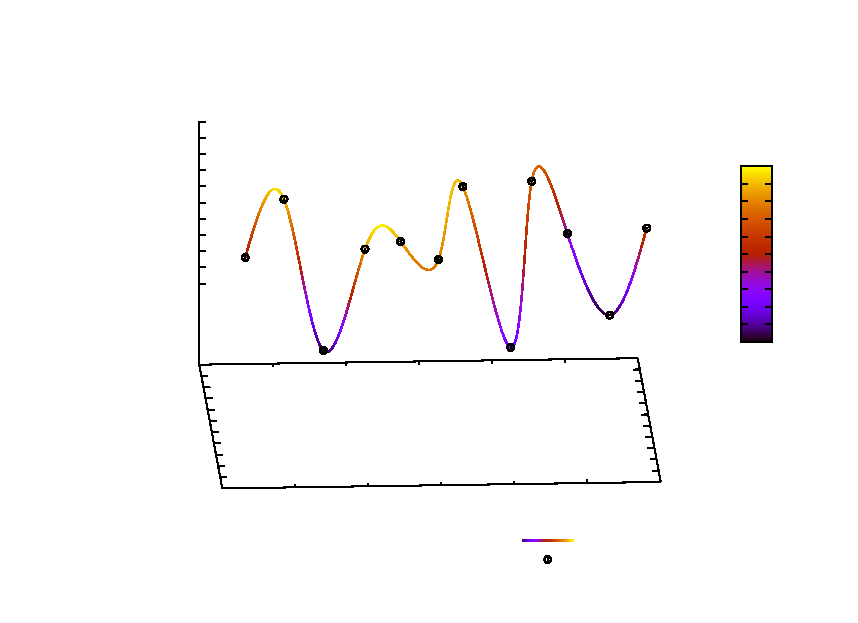
\includegraphics{./../LaTeX/graph/quest9-2}}%
    \gplfronttext
  \end{picture}%
\endgroup

	\caption{Interpolação com splines 3D - outro ângulo }
	\label{fig:quest9-2}
	\end{subfigure}
	\caption{Gráficos da questão 9}
\end{figure}
\FloatBarrier
